\chapter{Разбиение ребер двудольного графа на паросочетания}\label{akm1}

\section{Введение}
Использованы обозначения и определения книги \cite{akm-1}.
Исходные данные к расписанию обслуживания в заданной системе <<приборов>> $X$ множества <<требований>> $Y$ представлены двудольным графом\ ${G=(X,Y,E)}$. Прибору\ $x_i$\ планируется выполнение операции над требованием\ $y_j$ тогда  и только тогда, когда множество ребер\ $E$\ содержит ребро\ $(x_i,y_j)$. Одновременное участие объекта (прибора/требования) в двух и более операциях запрещено, длительность каждой операции равна 1, порядок выполнения операций безразличен, отношение частичного предшествования отсутствует. Построить расписание означает тем или иным способом указать для каждого ребра\ $(x_i,y_j )\in E$\ промежуток времени единичной длины, когда прибор $x_i$ обслуживает требование $y_j$.
\par\medskip
Биекция множества пронумерованных ($0, 1,\dots $)\  дискретных промежутков времени
$$
(0,1], (1,2], \dots
$$
в множество цветов с аналогичными номерами сводит задачу построения расписания к задаче о правильной реберной раскраске графа. Задача о расписании минимальной длительности эквивалентна задаче о правильной реберной раскраске графа $G$ в цвета $0, 1,\dots, \chi^\prime(G)-1 $,\ где\ $\chi^\prime(G)$ --- реберное хроматическое число графа $G$. Известный результат Г.\,Визинга \cite{akm-2} гласит, что в общем случае $\chi'(G)$\ равно\ $\Delta(G)$\ или\ $\Delta(G)+1$,\ где\ через $\Delta(G)$\ обозначена наибольшая степень вершины графа $G$. I.\,Holyer доказал \cite{akm-3}, что задача проверки равенства\ $\chi'(G)= \Delta(G)$\  NP-полна даже для случая кубических графов. Для случая двудольного графа, согласно теореме Д.\,Кенига о реберной раскраске \cite[c.\,80]{akm-4}, справедливо равенство $\chi'(G)=\Delta(G)$. Поэтому всюду в дальнейшем под расписанием, соответствующим графу\ $G$,\ будем подразумевать расписание длительности\ $\Delta(G)$. Расписание можно определить как разбиение множества\ $E$\ на\ $\Delta(G)$\ паросочетаний множества\ $X$\ с множеством\ $Y$:
\begin{equation}\label {eq01}
E_0,E_1,\dots, E_{\Delta(G)-1},
\end{equation}
где паросочетание\ $E_i$\  задает информацию о взаимодействии объектов в момент времени\ $i$;\ $0\leqslant i\leqslant \Delta(G)-1$.

Теорема Д.\,Кенига о реберной раскраске доказывает существование расписания, но не предлагает способ построения расписания с теми или иными свойствами, полезными для приложений. Особый интерес для приложений представляют такие расписания, где все приборы работают непрерывно с момента одновременного включения, причем прибор\ $i$ выключается точно по истечении\ $d_G x_i$ единиц времени. Другими словами, такие разбиения \eqref{eq01} множества ребер графа \ $G=(X,Y,E)$,\ где для каждой вершины $x_i\in X$ степени\ $k$ каждое из паросочетаний \ $E_0,E_1,\dots, E_{k-1}$\ содержит ребро, инцидентное вершине\ $x_i$. Разбиение \eqref{eq01}, обладающее таким свойством, будем называть \textit{ последовательным}.
\par\medskip
Получены условия существования последовательного разбиения. Последовательные разбиения востребованы в задачах составления расписаний минимальной длительности с беспростойной работой каждого прибора с момента включения вплоть до его выключения (все приборы включаются одновременно). Например, лекторы основного вуза могут совмещать основную работу с дополнительной работой в филиале, и от диспетчера расписания основного вуза требуется составить расписание таким образом, чтобы лекции каждого <<совместителя>> располагались в начале расписания и проводились без <<окон>> для лектора.
%\par\medskip
\section{Условия существования полного паросочетания в двудольном графе}
%\par\smallskip

Паросочетание в двудольном графе\ $G=(X,Y,E)$, насыщающее все вершины $X$, называется \textit{ полным паросочетанием} $X$ с $Y$.
Необходимые и достаточные условия существования в двудольном графе $G=(X,Y,E)$ полного паросочетания $X$  с $Y$  формулируются в известной теореме Холла \cite[c.\,164]{akm-1}:
\begin{equation}\label {eq02}
|A| \leqslant |\Gamma(A)|\quad \forall A\subseteq X,
\end{equation}
где\ $\Gamma(A)$ ---  множество вершин, смежных вершинам $A$.

Проверка условий затрудняется требованием выполнения неравенства \eqref{eq02} для каждого подмножества из $X$. Поэтому имеет смысл поиск условий, допускающих простую проверку. Известно, например \cite[c.\,165]{akm-1}, что в двудольном графе \ ${G=(X,Y,E)}$\  существует полное паросочетание\ $X$\  с\ $Y$,\ если
%\begin{equation}
$$
\min_{x\in X} d_{G}x\geqslant \max_{y\in Y}d_{G}y.
$$
%\end{equation}
Последнее равносильно выполнению для всех вершин\ ${x\in X},\ {y\in Y}$\ неравенства:
$$
d_G x\geqslant d_G y.
$$
Избыточность условия особенно заметна применительно к двудольному графу из нескольких компонент: соотношения между степенями вершин, принадлежащих разным компонентам графа, очевидно, не должны влиять на существование полного паросочетания.
\par\medskip
\begin{lemma}\label{lem01}
Пусть задан двудольный граф\ ${D=(A,B,C)}$, где\ $A$\ и\ $B$\ --- множества вершин,\ $C$ --- множество ребер. Если для каждого ребра\ $(a_i,b_j)\in C$\ справедливо неравенство\
\begin{equation}\label {eq00}
d_D a_i\geqslant d_D b_j,
\end{equation}
то\ $|A|\leqslant |B|$.
\end{lemma}
%\par\medskip
\begin{theorem}\label{the01}
В двудольном графе\ $G=(X,Y,E)$\ существует полное паросочетание\ $X$\ с\ $Y$, если для каждого ребра\ $(x,y)\in E$\  $(x\in X, y\in Y)$\ выполняется неравенство\ $d_G x\geqslant d_G y$.
\end{theorem}
\section{Наследуемые свойства и последовательные разбиения}
%\par\smallskip
Паросочетание в двудольном графе\ $G=(X,Y,E)$, насыщающее все вершины степени $\Delta(G)$, при этом в множестве $X$ --- только вершины степени $\Delta(G)$,  будем называть \textit{ минимаксом} графа\ $G$.
Будем говорить, что двудольный граф\ $G=(X,Y,E)$\ обладает свойством \textit{ жесткой асимметрии}, если
\begin{equation}\label{eq04}
d_G x\geqslant d_G y \text{ для каждого ребра } (x,y)\in E, \quad x\in X,\  y\in Y.
\end{equation}
\begin{lemma}\label{lem02}
Двудольный граф\ $G=(X,Y,E)$\ со свойством жесткой асимметрии обладает минимаксом.
\end{lemma}
Пусть $P$ --- некоторое свойство двудольного графа\ ${G=(X,Y,E)}$, достаточное для существования минимакса у графа $G$. Свойство\ $P$ будем называть \textit{ наследуемым}, если выполнение свойства\ $P$\ для графа\ $G$\ влечет выполнение свойства\ $P$\ для каждого потомка 1-го уровня.
\begin{remark}\label{rem01}
 Если граф\ $G$\ обладает наследуемым свойством, то каждый потомок графа $G$ обладает минимаксом.
\end{remark}
\begin{theorem}\label{the02}
 Свойство жесткой асимметрии является наследуемым свойством.
 \end{theorem}
\begin{theorem}\label{the03}
 Если двудольный граф\ $G=(X,Y,E)$\ обладает наследуемым свойством, то последовательное разбиение существует.
\end{theorem}
\begin{remark}\label{rem02}
Из Теорем 2 и 3 видно, что для двудольного графа\ ${G=(X,Y,E)}$ со свойством жесткой асимметрии существует последовательное разбиение.
Данный результат был получен ранее в работе \cite{akm-5} с использованием принципиально другого подхода.
\end{remark}

Рассмотрим для двудольного графа\ ${G=(X,Y,E)}$ свойство:
\begin{equation}\label{eq05}
d_G{x_1} + d_G x_2\geqslant d_G y_1+d_G y_2\ \text{ для каждой пары ребер }\  (x_1,y_1)\ \text{ и }\ (x_2,y_2).
\end{equation}
Свойство \eqref{eq05} будем называть \textit{ мягкой асимметрией}. Очевидно, что \eqref{eq05} следует из \eqref{eq04}, но свойство \eqref{eq05} может выполняться и в ситуации, когда \eqref{eq04} нарушено.

\begin{theorem}\label{the05}
Если двудольный граф\ $G=(X,Y,E)$ обладает свойством мягкой асимметрии, то последовательное разбиение существует.
\end{theorem}
\section{ Заключение}
Перспективным представляется направление поиска условий существования расписаний рассмотренного выше типа, но без требования одновременного включения приборов. В общем случае задача о существовании таких расписаний является NP-полной \cite{akm-6}.  Для одного частного случая условия существования расписания длительности 5 получены в \cite{akm-7}, алгоритм их проверки изложен в \cite{akm-8}.  Для случая, когда степень каждой вершины множества\ $X$\ равна\ $\Delta(G)$, $\Delta(G)-2$ или 2, задача рассмотрена в \cite{akm-9}.
\par\medskip



\chapter{Алгоритмы построения и оптимизации двух типов расписаний}\label{akm2}
\section{Введение}
В исследованиях задач составления расписаний учебных занятий
\cite[с.\,403]{akm-1}, их приведения к «безоконному» виду \cite{akm-5}, а также в задачах о расписаниях обслуживания множества заданий в мультипроцессорной системе без простоя процессоров и прерываний обработки каждого задания \cite{akm-3Tanaev} нередко используются методы теории графов.
\par\medskip
Пусть $G=(V,E)$ --- связный граф. Цепью в\ $G=(V,E)$\ называется такая последовательность вершин\ $a_i$ и попарно различных ребер $b_i$ (вершины могут повторяться)
\begin{equation}\label{eq1}
P_0=(a_0,b_0,a_1,b_1,…,b_{k-1},a_k), 			
\end{equation}
что каждые два соседних ребра $b_{i-1}$ и $b_i$ имеют общую вершину $a_i$; если все вершины в (\ref{eq1}) попарно различны, то цепь называется простой. Если концевые вершины  $a_0$ и $a_n$ (простой) цепи (\ref{eq1}) совпадают, то (простая) цепь (\ref{eq1}) называется (простым) циклом. В настоящей статье обсуждается использование цепочечных структур (цепей и конкатенаций нескольких цепей): в разделе \ref{akm-ss1} --- для построения однопроцессорного расписания с условиями предшествования, в разделе \ref{akm-ss3} -- для проверки существования интервальной реберной раскраски двудольных графов -- графической интерпретации многопроцессорного расписания без простоев и без условий предшествования.
\par\medskip
Интервальной реберной раскраской графа\ {G=(V,E)}\ называется такое отображение множества ребер\ $E$\ в множество целых чисел (<<цвета>>), при котором для каждого\ $v$\ из множества вершин\ $V$\ цвета ребер, инцидентных\ $v$, различны и образуют целочисленный интервал (далее будем писать кратко: <<интервальная раскраска>>).
\par\medskip
Примеры.

1) Простой цикл нечетной длины не имеет интервальной раскраски.

2) Простой цикл четной длины интервально раскрашиваем.

Задача об интервальной раскраске заданного графа\ $G=(V,E)$ $NP$-полна \cite{akm-2}. Свойство $NP$-полноты сохраняется и в случае двудольного графа \cite{akm-8Seva}. Сложность задачи об интервальной раскрашиваемости может различаться для разных классов двудольных графов. Ниже показано, что любой регулярный двудольный граф допускает интервальную раскраску (результат Р.\,Камаляна \cite{akm-9Kamal}), при этом задача об интервальной раскрашиваемости обыкновенного регулярного графа $NP$-полна \cite{akm-2}).
\par\medskip
Общеизвестно, что текстуально близкие задачи теории графов нередко принадлежат разным классам сложности. Из примеров, приведенных в \cite[с.\,104]{akm-10Geri}, для целей нашей статьи уместно указать на следующие две задачи: <<Кратчайший путь между двумя вершинами>> и <<Самый длинный путь между двумя вершинами>> в заданном графе $G=(V,E)$; первая, как известно, разрешима за время $O(|V|^2)$, вторая же $NP$-полна -- к этой задаче сводится задача <<Гамильтонов путь между двумя вершинами>> \cite[с.\,269]{akm-10Geri}.
\par\medskip
\begin{remark}\label{lab1}
 Для задачи <<Кратчайший путь между двумя вершинами>> неизвестен алгоритм с оценкой $O(|E|)$, см. \cite[c.\,236]{akm-11Aho}.
\end{remark}
\par\medskip
Сложность задачи о гамильтоновом маршруте (цикле или пути) принципиально различна для графов разных классов. Рассмотренные в следующем разделе задачи тесно связаны с вычислением гамильтоновых маршрутов в графах простой структуры: в связном регулярном графе четной степени и ациклическом ориентированном графе.
\par\medskip
\section{Расписание выполнения заданий в однопроцессорной системе с условиями частичного предшествования}\label{akm-ss1}
\label{sec1}
\subsubsection{Достаточные условия интервальной раскрашиваемости}\label{subsec11}
 Из теоремы Эйлера %\cite[c.\,192]{akm-7Emel}
  следует, что связный регулярный граф $G$\ четной степени обладает эйлеровым циклом (под степенью регулярного графа будем понимать степень вершины графа); теорема Ю.\,Петерсена \cite{akm-12Petersen} утверждает, что связный регулярный граф четной степени $2n$ допускает разложение на $n$\ $2$-факторов (каждая связная компонента $2$-фактора является гамильтоновым циклом). Если каждый из этих $2$-факторов является набором циклов четной длины в графе $G$, то, помечивая последовательные ребра каждого цикла $i$-го набора метками
$$
  2i,2i+1,2i,2i+1,...  (i=0,1,…,n-1),
$$
можно получить интервальную раскраску.
Из перечисленных свойств графа сохраним лишь требование четности длины любого цикла. Но последнее, согласно теореме Кенига, означает двудольность графа, а как уже отмечалось ранее, не всякий двудольный граф интервально раскрашиваем. Более того, проверка интервальной раскрашиваемости является $NP$-полной задачей, следовательно, не существует эффективно проверяемых необходимых и достаточных условий (в предположении истинности гипотезы $P\neq NP$). Поэтому для обеспечения свойства интервальной раскрашиваемости следует добавить некоторое дополнительное условие (разумеется, менее слабое, чем регулярность с четной степенью). Потребуем выполнение свойства регулярности без условия четности степени графа $\Delta$.
\par\medskip
В случае нечетного $\Delta$ достаточно найти в заданном регулярном двудольном графе $G=(X,Y,E)$ полное паросочетание $X$ c $Y$ (существование такого паросочетания следует из следствия 8.16.1 \cite[с.\,165]{akm-1}), раскрасить его ребра цветом $\Delta-1$ и удалить его, затем воспользоваться теоремой Ю.\,Петерсена для интервальной раскраски оставшегося графа $\Delta-1$ цветами: $0, 1, \dots, \Delta-2$. Таким образом, мы пришли к известному результату \cite{akm-9Kamal} об интервальной раскрашиваемости любого регулярного двудольного графа.
\par\medskip
\subsubsection{Перечисление допустимых расписаний с условиями частичного предшествования}
\label{subsec12}
Пусть однопроцессорной системе выделены для обработки объекты $0,1,\dots,n-1$ и заданы условия частичного предшествования: для некоторых пар объектов указано, что один из объектов пары должен быть обработан раньше другого. Требуется построить допустимое расписание обработки, другими словами, упорядочить все объекты в соответствии с условиями частичного предшествования.
Рассмотрим орграф $G=(V,E)$, вершины $v_0,v_1\dots,v_{n-1}$ которого соответствуют заданным объектам, дуги -- условиям частичного предшествования: из вершины $v_i$ в вершину $v_j$ дуга проведена тогда и только тогда, когда объект с номером $j$ предшествует объекту с номером $i$. Если в орграфе $G$ имеется цикл, то искомое расписание, очевидно, не существует (ориентированный граф имеет цикл в том и только в том случае, когда алгоритм поиска в глубину находит обратную дугу \cite{akm-13Tucker}). Если $G$ – ациклический орграф, то для построения допустимого расписания достаточно применить алгоритм топологической сортировки (см. \cite[с.\,96]{akm-1}). Мы предложим близкий по идее алгоритм, на основе которого удается не только построить допустимое расписание, но и выполнить перечисление таких расписаний.
\par\medskip
\textbf{ Алгоритм 1 (иерархическая сортировка вершин графа)}
\par\smallskip
\textbf{ Вход: } связный ациклический орграф  $G=(V,E)$ на $n$ вершинах.

\textbf{ Выход: } такая упорядоченная последовательность $T$ вершин множества $V$, что для каждой дуги ${(v_i, v_j)\in E}$ вершина $v_j$ предшествует вершине $v_i$ в последовательности $T$.

 \textbf{ Обозначения: } $m(v)$ -- целочисленные метки вершин ${v\in V}$; $L[i]$ -- список всех вершин с $i$ исходящими дугами, $i=0, 1, \dots, n-1$ (вначале все списки пусты).
\par\medskip
1. Для каждого $v\in V$ выполнить:

\{

$m(v):=0;\ i:= d^-(v);$\ добавить $v$ в $L[i]$;

\}

2. \textbf{ Пока} $E\neq \varnothing$, выполнить:

	\{
	
		2.1. выбрать произвольную вершину $v$ из $L[0]$ и дугу $(u,v)$;
		
		2.2. \textbf{ если} $m(v)+1>m(u)$, \textbf{ то} $m(u):=m(v)+1$;
		
		2.3. $i:=d^-(u)$;
		
		2.4. удалить дугу $(u,v)$ из $E$;
		
		2.5. переместить вершину $u$ из $L[i]$ в $L[i-1]$;
		
		2.6. \textbf{ если} $d^+(v)=0$, \textbf{ то} удалить вершину $v$ из графа и из $L[0]$;
	
\}

3. Восстановить исходный граф ${G=(V,E)}$.

4. ${m_0:=\max_{v\in V} m(v)}$.

5. $T:=\varnothing$.

6. Для $i=0,\dots, m_0$ выполнить:

\{

6.1. для каждого $v\in V$ выполнить:

6.1.1. \textbf{ если} $m(v)=i$, \textbf{ то} добавить $v$ к концу последовательности $T$;

\}

\textbf{ Конец Алгоритма 1}
\par\medskip
Нетрудно видеть, что сложность Алгоритма 1 не превышает $O(n^2)$.

\begin{state}\label{state1} Упорядочение объектов, индуцированное последовательностью $T$, является допустимым расписанием.
\end{state}
\begin{proof}
 Отсутствие вершины с нулевой полустепенью исхода в орграфе $G$ (или в подграфе, полученном в каждой итерации цикла) означало бы присутствие в орграфе цикла, что противоречит условию применения иерархической сортировки.

Для каждой дуги $(v_i,v_j)$ метка, присваиваемая вершине $v_i$ алгоритмом иерархической сортировки, превышает метку, присваиваемую вершине $v_j$:\ ${m(v_i)\geq m(v_j)+1}$. Следовательно, если известно, что $j$-й объект предшествует $i$-му объекту, то в списке объектов, индуцированном последовательностью $T$, объект с номером $j$ располагается раньше объекта с номером $i$, т.е. получено допустимое расписание.
\end{proof}
В следующем следствии через $V_i$ обозначено множество всех вершин $v$ с меткой ${m(v)=i}$, ${i=0,\dots, m_0}$.
\begin{corollary}
Количество допустимых расписаний равно $|V_0|!\dots|V_{m_0}|!$
\end{corollary}
\begin{remark}
Задача иерархической сортировки текстуально близка к задаче поиска ориентированного гамильтонова пути в каждой компоненте ориентированного графа. Уже отмечалось, что в общем случае задача о гамильтоновом пути $NP$-полна, но для ациклических ориентированных графов задача разрешима за полиномиальное время \cite{akm-14Lawler}.
\end{remark}

\begin{figure}[H]
{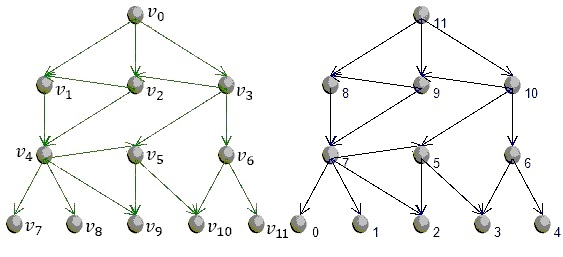
\includegraphics[width=15cm,height=7cm, keepaspectratio]{02}}
{\small %временный переход к мелкому шрифту
\hspace{4cm}(а) \hspace{8cm} (б)\\
}
\caption{(а) Орграф $G$;\ (б) результат Алгоритма 1 -- вершины орграфа $G$ упорядочены по неубыванию меток.}
\label{akmfig2}
\end{figure}
%$$
%\includegraphics[width=15cm,%
%height=7cm, keepaspectratio]%
%{02}
%$$
%%\hspace{-0.8cm}
%\begin{minipage}[t]{0.99\hsize} %вложенная надпись
%{\small %временный переход к мелкому шрифту
%\hspace{3cm}(а) \hspace{8cm} (б)\\
%$\phantom{--}$ Рис.\,2. (а) Орграф $G$;\ (б) результат Алгоритма 1 -- вершины орграфа $G$ упорядочены по неубыванию меток.\\
%}
%\end{minipage}%завершение вложенной надписи
\par\medskip
Рассмотрим пример. Пусть $n=12$, для каждого объекта в скобках указаны предшествующие ему объекты: 0 (1, 2, 3), 1(4), 2(1, 4), 3(2, 5, 6), 4(5, 7, 8, 9), 5(9, 10), 6(10, 11). В частности, отсюда видно, что объекту 3 предшествуют объекты 2, 5 и 6, а у объектов 7,$\dots$, 10 нет предшественников. На рис.\,\ref{akmfig2}а приведен орграф $G$.
\begin{figure}[H]
{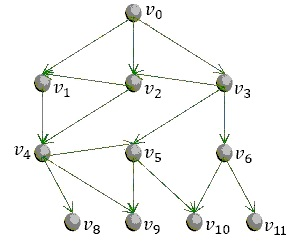
\includegraphics[width=15cm,height=7cm, keepaspectratio]{03}}
\caption{Первая итерация цикла 2 Алгоритма 1.}
\label{akmfig3}
\end{figure}
%$$
%\includegraphics[width=15cm,%
%height=7cm, keepaspectratio]%
%{03}
%$$
%%\hspace{-0.8cm}
%\begin{minipage}[t]{0.99\hsize} %вложенная надпись
%{\small %временный переход к мелкому шрифту
%
%$\phantom{--}$ Рис.\,3. Первая итерация цикла 2 Алгоритма 1.\\
%}
%\end{minipage}%завершение вложенной надписи
\par\medskip\medskip
На рис.\,\ref{akmfig3} отображены результаты выполнения первой итерации цикла 2, где: выбраны вершина ${v_7\in L[0]}$ и дуга ${(v_4,v_7)}$; метке ${m(v_4)}$ присвоено значение 1, переменной $i$ -- значение 2; дуга ${(v_4,v_7)}$ удалена; вершина $v_4$ перемещена из $L[2]$ в $L[1]$; вершина $v_7$ удалена из графа и из $L[0]$.
%$$
%\includegraphics[width=15cm,%
%height=7cm, keepaspectratio]%
%{04}
%$$
%%\hspace{-0.8cm}
%\begin{minipage}[t]{0.99\hsize} %вложенная надпись
%{\small %временный переход к мелкому шрифту
%
%$\phantom{--}$ Рис.\,4. Вторая итерация цикла 2 Алгоритма 1.\\
%}
%\end{minipage}%завершение вложенной надписи
%\par\medskip
\begin{figure}[H]
{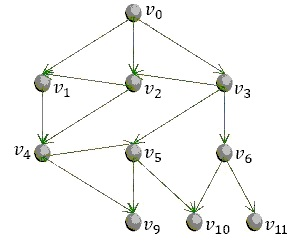
\includegraphics[width=15cm,height=7cm, keepaspectratio]{04}}
\caption{Вторая итерация цикла 2 Алгоритма 1.}
\label{akmfig4}
\end{figure}
\par\medskip\medskip
Во второй итерации цикла 2 (рис.\,\ref{akmfig4}) для вершины $v_8$ выполнены действия, аналогичные выполненным ранее для вершины $v_7$. Окончательный результат выполнения Алгоритма 1 приведен на рис.\,\ref{akmfig2}б.

\section{Жадный алгоритм интервальной раскраски}\label{akm-ss3}
\subsubsection {Кусочно-непрерывный путь}\label{akm-ss4}
\label{subsec21}
Цепь (\ref{eq1}) в графе $G$ называется непродолжимой, если $P_0$ содержит все ребра графа $G$, инцидентные вершине $a_k$. Обозначим через $G'$ копию графа $G$ и определим кусочно-непрерывный путь в $G$ следующим образом.

Пока имеется ребро графа $G'$, не входящее в $P_0$, выполним действия: для графа, полученного удалением из $G'$ всех ребер, включенных в $P_0$, сохраним обозначение $G'$ и выберем $a_k$ -- самую правую из вершин $P_0$, имеющих в графе $G'$ инцидентные ребра; построим в графе $G'$ непродолжимую цепь $P_1$, начинающуюся с вершины $a_k$, затем выполним конкатенацию $P_0$ и цепи $P_1$ и обозначим результат конкатенации через $P_0$.
Последовательность ребер графа $G$, перечисленных в том порядке, в каком они следуют в последнем $P_0$, будем называть кусочно-непрерывным путем в графе $G$ и обозначать через $P$. Очевидно, кусочно-непрерывных путей в графе $G$ может быть несколько.
\par\medskip
Поясним на примере графа $G$, приведенного на рис.\,\ref{akmfig5}а. Выберем в $G$ непродолжимую цепь
${P_0=(a_0,b_0,}{a_4,b_1,a_1,}{b_2,a_5,b_3,}{a_0,b_4,a_7,}{b_5,a_2,}{b_6,a_4)}.$
Затем удалим из копии $G'$ графа $G$ ребра $b_0,\dots,b_6$, включенные в $P_0$. Самой правой вершиной $P_0$, обладающей в оставшемся графе $G'$ инцидентными ребрами, будет вершина $a_2$ (инцидентные ребра: $b_7$ и $b_8$). Построим в $G'$ непродолжимую цепь $P_1= (a_2,b_7,a_5)$; для результата конкатенации $P_0$ и $P_1$ сохраним обозначение $P_0$:
${P_0=(a_0,b_0,}{a_4,b_1,a_1,}{b_2,a_5,b_3,}{a_0,b_4,a_7,}{b_5,a_2,b_6,}{a_4;}{ a_2,b_7,a_5)}$
и удалим из графа $G'$ ребро $b_7$. Самой правой вершиной $P_0$, обладающей инцидентными ребрами, снова является вершина $a_2$, ${P_1= (a_2,}{b_8,a_{11},}{b_9,a_3,}{b_{10},a_6,}{b_{11},a_1,b_{12},}{a_8,b_{13},}{a_3,b_{14},a_7)}$ -- непродолжимая цепь графа $G'$, начинающаяся в вершине $a_2$. Результат конкатенации $P_0$ и $P_1$ обозначим через $P_0$:
${P_0=(a_0,b_0,}{a_4,b_1,}{a_1,b_2,}{a_5,b_3,}$ ${a_0,b_4,}$ ${a_7,b_5,}{a_2,b_6,a_4;}$ ${a_2,b_7,a_5;}$ $
{a_2,b_8,}$ ${a_{11},b_9,}{a_3,b_{10},}$ ${a_6,}$ ${b_{11},}$ ${a_1,b_{12},}$ ${a_8,b_{13},}{a_3,b_{14},}{a_7)}$.
Непродолжимая цепь, начинающаяся в вершине ${a_3:}$ ${P_1 = (a_3,}$ ${b_{15},a_9,}$ ${b_{16},a_1)}$. Выполним конкатенацию с $P_0$, после чего в качестве заключительного шага выберем непродолжимую цепь ${P_1=(a_3,}$ ${b_{17},a_{10})}$ и выполним ее конкатенацию с $P_0$. В результате получим кусочно-непрерывный путь в графе ${G: P=(b_0,}$ ${b_1,\dots,b_{17})}$.
\par\medskip
\begin{remark} Естественным представляется вместо <<просто>> непродолжимой цепи рассматривать самую длинную цепь в графе. Однако, как отмечено выше, ее построение затруднено $NP$-полнотой соответствующей задачи распознавания.
\end{remark}

\begin{figure}[H]
{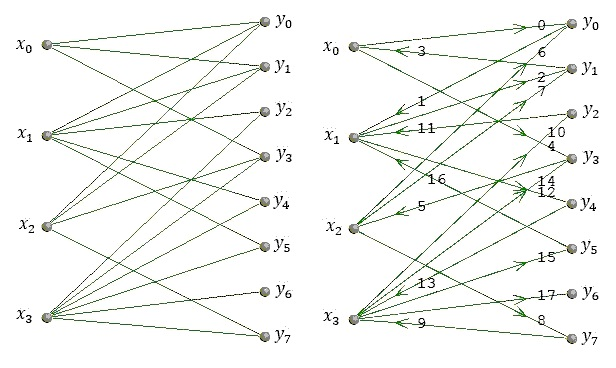
\includegraphics[width=15cm,height=7cm, keepaspectratio]{05}}
{\small %временный переход к мелкому шрифту
\hspace{-10cm}(а)\hspace{5cm}(б)}
\caption{(а) Двудольный граф $G=(X,Y,E)$, $|X|=4,|Y|=8;$\
 (б) кусочно-непрерывный путь $P$, полученный компьютерным путем. Номера ребер соответствуют порядку их следования в $P$.}
\label{akmfig5}
\end{figure}
\par\medskip
%$$
%\includegraphics[width=15cm,%
%height=7cm, keepaspectratio]%
%{05}
%$$
%%\hspace{-0.8cm}
%\begin{minipage}[t]{0.99\hsize} %вложенная надпись
%{\small %временный переход к мелкому шрифту
%\hspace{3cm}(а) \hspace{8cm} (б)\\
%$\phantom{--}$ Рис.\,5. (а) Двудольный граф $G=(X,Y,E)$, $|X|=4,|Y|=8;$\
% (б) кусочно-непрерывный путь $P$, полученный компьютерным путем. Номера ребер соответствуют порядку их следования в $P$.\\
%}
%\end{minipage}%завершение вложенной надписи
%\par\medskip
\subsubsection {Жадный алгоритм интервальной раскраски}
\label{subsec22}
Пусть в двудольном графе ${G=(V,E)}$, ${V=(X,Y)}$, ${|E|=m},{|V|=n}$, построен кусочно-непрерывный путь $P$ из последовательных ребер ${e_i= (v_i,w_i)}$, $i=0\dots,m-1$. В прикладных задачах нередко требуется построить интервальную раскраску, удовлетворяющую дополнительному условию -- все цвета принадлежат некоторому <<допустимому>> диапазону. Допустимый для раскрашивания ребер диапазон цветов обозначим через $[-t..t]$, где $t$ -- заданное целое положительное число. Цвет ребра $e_i$ будем обозначать $C[i]$, $i= 0, \dots, m-1$. Цвета всех раскрашенных ребер, инцидентных вершине $v_i$, будем называть цветами, \textit{ представленными в вершине} $v_i$; для их хранения используем список $L[v_i]$, ${i=0, \dots, n-1}$.
\par\medskip
Предлагается раскрасить последовательные ребра кусочно-непрерывного пути $P$ цветами из допустимого диапазона так, чтобы в каждый момент времени для каждой вершины $v_i$ цвета, представленные в $v_i$, составляли (целочисленный) интервал. Алгоритм раскрашивания, обладающий таким свойством, будем называть \textit{ жадным алгоритмом}.
\par\medskip
Для заданного непустого целочисленного интервала цветов ${[a..b] =}$ ${a,a+1,\dots,b}$ цвета из множества $\{a-1, b+1\}
\cap {[-t..t]}$ будем называть \textit{ приграничными цветами}; для пустого интервала приграничным цветом считается каждый цвет из допустимого диапазона.
Для ребра $e_i=(v_i,w_i)$ через ${M_1=}{[min_1..max_1]}$ и ${M_2=}{[min_2..max_2]}$ будем обозначать интервалы цветов, представленных в вершинах $v_i$ и  $w_i$, $M_1'$ и $M_2'$ -- множества цветов, приграничных для $M_1$ и $M_2$ соответственно. Из соображений краткости мы не будем снабжать эти обозначения индексом $i$, поскольку всюду в дальнейшем индекс $i$ однозначно определяется из контекста.

\begin{state}\label{St2}
Пусть ребро $e_i=(v_i,w_i)$ не раскрашено. Для раскраски ребра $e_i$ в соответствии с жадным алгоритмом может быть выбран любой цвет из пересечения
$M_1'\cap M_2'$ и никакой другой.
\end{state}
\begin{proof}
Справедливость утверждения следует из того, что жадный алгоритм сохраняет свойство интервальности как для цветов, представленных в вершине $v_i$, так и для цветов, представленных в вершине  $w_i$.
 %Доказательство закончено.
\end{proof}
Пусть заданный допустимый интервал $[-t..t]$ достаточно большой, списки цветов $L[v_i]$ и $L[w_i]$, представленных в концевых вершинах ребра ${e_i=(v_i,w_i)}$, образуют непустые интервалы $M_1$ и $M_2$ соответственно. Цвет $r \in M_1'\cap M_2'$, допустимый для раскрашивания ребра $e_i$, может: 1) отсутствовать (например, при $M_1=[1..2]$, $M_2=[5..10]$), 2) определяться однозначно (например, $r=3$ при $M_1=[1..2]$, $M_2=[4..5]$), 3) принимать одно из двух значений (например, при $M_1=M_2=[3..4]$ можно выбрать $r=2$ или $r=5$).

Для формулировки Алгоритма 2 нам понадобится способ перебора <<состояний>> поиска допустимого цвета для рассматриваемого ребра $e_i$: $0, 1, \dots$; текущее состояние ребра ${e_i= (v_i,w_i)}$ будем обозначать через $q_i$; логическое условие, выражающее взаимное расположение интервалов  $M_1$ и $M_2$ (и случаи, когда один или оба интервала $M_1$ и $M_2$ пусты), будем обозначать через $p_i[q_i]$; цвет,  выбираемый для присвоения ребру $e_i$ в зависимости от $p_i[q_i]$ -- через $c_i[q_i]$.

При принятом здесь подходе количество таких <<состояний>> равно девяти. Соотнесем каждому $q_i=0, 1, \dots, 8$ соответствующие $p_i[q_i]$   и   $c_i[q_i]$.

\vspace{6pt}
\hspace{5cm} {\textit{ Список состояний:}}
\vspace{-6pt}
\begin{align*}
   &p_i[0]:=(L[v_i]=\varnothing) \,\&\, (L[w_i]=\varnothing);    && c_i[0]:=0;\\
  &p_i[1]:=(L[v_i]=\varnothing) \,\&\, (L[w_i]\neq \varnothing) \,\&\, ( min_2>-t); &&c_i[1]:=min_2-1;\\
   &p_i[2]:=(L[v_i]=\varnothing) \,\&\, (L[w_i]\neq \varnothing) \,\&\, ( max_2<t);  &&c_i[2]:=max_2+1;\\
  &p_i[3]:=(L[v_i]\neq \varnothing) \,\&\, (L[w_i]=\varnothing) \,\&\, ( min_1>-t); &&c_i[3]:=min_1-1;\\
   &p_i[4]:=(L[v_i]\neq \varnothing) \,\&\, (L[w_i]=\varnothing) \,\&\, ( max_1<t);  &&c_i[4]:=max_1+1;\\
   &p_i[5]:=(L[v_i]\neq \varnothing) \,\&\, (L[w_i]\neq \varnothing) \,\&\, ( min_1>-t) \,\&\, (min_1=min_2); &&c_i[5]:=min_1- 1;\\
   &p_i[6]:=(L[v_i]\neq \varnothing) \,\&\, (L[w_i]\neq \varnothing) \,\&\, ( max_1=max_2) \,\&\, (max_1<t);  &&c_i[6]:=max_1+1;\\
   &p_i[7]:=(L[v_i]\neq \varnothing) \,\&\, (L[w_i]\neq \varnothing) \,\&\, ( max_1+2=min_2); &&c_i[7]:=max_1+1;\\
  &p_i[8]:=(L[v_i]\neq \varnothing) \,\&\, (L[w_i]\neq \varnothing) \,\&\, ( max_2+2=min_1); &&c_i[8]:=max_2+1;
\end{align*}
Например, для ребра ${e_i=(v_i,w_i)}$ при $q_i=8$ условие $p_i[q_i]$:
$$(L[v_i]\neq \varnothing)\ \&\ (L[w_i]\neq \varnothing)\ \&\ (max_2+2=min_1),$$
означает, что списки цветов, представленных в вершинах $v_i$ и  $w_i$ соответственно, не пусты, интервал $M_2$ располагается на числовой оси левее интервала $M_1$, при этом наибольшее значение ($max_2$) из интервала $M_2$ на две единицы меньше наименьшего значения ($min_1$) из интервала $M_1$. Поэтому множество $M_1'\cap M_2'$ цветов, приграничных как для $M_1$, так и для $M_2$, содержит единственный элемент, равный $max_2+1$. Понятно, что он и выбирается в качестве цвета, присваиваемого ребру $e_i$: $c_i[8]:=max_2+1$.
\par\medskip
В основе Алгоритма 2 лежит идея перебора с возвратами. Каждая итерация цикла по раскрашиванию ребер $e_i (i=0,\dots n-1)$ состоит из двух шагов -- прямого и возвратного.
Прямой шаг включает действия по раскрашиванию ребра $e_i=(v_i,w_i)$ кусочно-непрерывного пути $P$ с сохранением цветов предшествующих ребер. Возвратный шаг выполняется, когда прямой шаг по раскрашиванию очередного ребра $e_i$ не увенчался успехом, и включает действия по изменению цветов некоторых ребер, предшествующих $e_i$, с целью подготовить условия для успешного раскрашивания ребра $e_i$.
Нумерация ребер соответствует порядку их следования в кусочно-непрерывном пути $P$.
\par\medskip
\textbf{ Алгоритм 2 (жадный алгоритм интервальной раскраски)}
\par\smallskip
\textbf{ Вход: } $G=(V,E)$ -- связный двудольный граф, $|V|=n, |E|=m$;

кусочно-непрерывный путь $P$ в графе $G$;
%
%$[-t..t]$ -- допустимый диапазон цветов;

\textbf{ Выход: }
Массив $C[0..m-1]$ для цветов ребер и логическая переменная $Success$; переменной $Success$ будет присвоено значение $true$ в случае, если интервальная раскраска получена, и значение $false$ -- в противном случае.
\par\smallskip
\noindent\textbf{ 1. Инициализация:}
\begin{itemize}
	\item [1.1.] Для $k=0, ..., m-1$ выполнить: $q_k:=-1$;
	\item [1.2.] Для $k=0, ..., n-1$ выполнить: $L[v_k]:=\varnothing$;
	\item [1.3.] $i:=0$;
\end{itemize}
\noindent\textbf{ 2. Прямой шаг:}
\begin{itemize}
	\item [2.1.] \textbf{ если} $q_i\geq 8$, \textbf{ то} переход к пункту \textbf{ Возвратный шаг};
	\item [2.2.] \textbf{ если} $L[v_i]\neq \varnothing$, \textbf{ то} переменным $min_1$ и $max_1$ присвоить соответственно минимальное и максимальное значения списка $L[v_i]$;
	\item [2.3.] \textbf{ если} $L[w_i]\neq \varnothing$, \textbf{ то} переменным $min_2$ и $max_2$ присвоить соответственно минимальное и максимальное значения списка $L[w_i]$;
	\item [2.4.] Для $k=q_i+1, \dots, 8$ выполнить: \textbf{ если} $p_i[k]=true^{*)}$, \textbf{ то}
	\{$q_i:=k$; переход к пункту 2.5\};\\
	переход к пункту \textbf{ Возвратный шаг};
	\item [2.5.]		$C[i]:=c_i[k]^{*)}$;\\
	  добавить $C[i]$ в списки $L[v_i]$ и $L[w_i]$;\\
		\textbf{ если} $i<m-1$, \textbf{ то} \{$i:=i+1;$ переход к пункту \textbf{ Прямой шаг}\}\\
		\textbf{ иначе} \{$Success:=true$;	завершить алгоритм\};
\end{itemize}
\noindent\textbf{ 3. Возвратный шаг:}
\begin{itemize}
	\item [3.1.] $q_i:=-1$;
	\item [3.2.] $i:=i-1$;
	\item [3.3.] \textbf{ если} $i=-1$, \textbf{ то} \{$Success:=false$; завершить алгоритм\};
	\item [3.4.] удалить $C[i]$ из $L[v_i]$ и $L[w_i]$;
	\item [3.5.] $q_i:=q_i+1$;
	\item [3.6.] переход к пункту \textbf{ Прямой шаг};
\end{itemize}

\textbf{ Конец Алгоритма 2}\\
---------\\
* Значения $p_i[k]$ и $c_i[k]$ см. в \textit{ Списке состояний}.
\par\medskip
Алгоритм 2 открывает перспективы для решения известной проблемы: верно ли, что любой двудольный граф с числом вершин $n=15,16,17,18$ допускает интервальную раскраску? Известно \cite{akm-15Giaro}, что при $n<15$ ответ положителен, а при $n>18$ -- отрицателен.

На рис.\,\ref{akmfig6} представлена интервальная раскраска, сгенерированная Алгоритмом 2 для двудольного графа, приведенного на рис.\,\ref{akmfig5}а. Время счета -- приблизительно 2\,мс на компьютере с характеристиками: $2.50\,GHz,\ 8.00\,GB$. Отметим, что первый возвратный шаг выполнен для ребра $e_7=(x_2, y_1)$, а общее число возвратных шагов составило $24$.
\begin{figure}[H]
\centerline{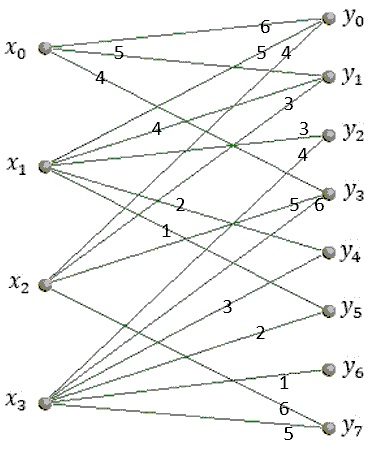
\includegraphics[width=15cm,height=7cm, keepaspectratio]{06}}
\caption{Интервальная раскраска графа ${G=(X,Y,E)}$, изображенного на рис.\,\ref{akmfig5}а, -- \vspace{-1mm} результат компьютерной реализации Алгоритма 2.}
\label{akmfig6}
\end{figure}
\par\medskip
%$$
%\includegraphics[width=15cm,%
%height=7cm, keepaspectratio]%
%{06}
%$$
%%\hspace{-0.8cm}
%\begin{minipage}[t]{0.99\hsize} %вложенная надпись
%{\small %временный переход к мелкому шрифту
%$\phantom{--}$ Рис.\,6. Интервальная раскраска графа ${G=(X,Y,E)}$, изображенного на рис.\,5а, -- \vspace{-1mm} результат компьютерной реализации Алгоритма 2.\\
%}
%\end{minipage}%завершение вложенной надписи
%\par\medskip
\section{Заключение}
Алгоритмы 1 и 2 воплощены в компьютерные программы, получены  свидетельства о государственной регистрации в Реестре программ для ЭВМ (2016 г.).
Из подраздела \ref{subsec12} видно, что алгоритм иерархической сортировки вершин имеет фактически линейную вычислительную сложность относительно длины входа. Вычислительные трудности жадного алгоритма интервальной раскраски коренятся в $NP$-полноте задачи распознавания об интервальной реберной раскрашиваемости двудольного графа. В худшем случае время работы данного алгоритма оценивается экспоненциальным образом, однако компьютерные эксперименты подтверждают его эффективность для практической работы с графами, в которых число вершин не превышает 20.

\chapter{Алгоритмическое и программное обеспечение}\label{akm3}
В соответствии с календарным планом, в 2016 г. планировалось создать алгоритмическое и программное обеспечение по некоторым вопросам оптимизации расписания для мультипроцессорных систем, которые тесно соприкасаются с вопросами оптимизации вузовского учебного процесса, представить на регистрацию в госпатенте не менее трех программ для ЭВМ. Результаты регистрации см. в \cite{akm-prog0} -- \cite{akm-prog5}.
\section{Разбиение множества ребер двудольного графа на непродолжимые реберно-пересекающиеся пути}

В задачах интервальных реберных раскрасок востребовано разбиение множества ребер двудольного графа на непродолжимые реберно-непересекающиеся пути, удовлетворяющее условию: для выбора начальной вершины очередного $i$-го пути $P[i] (i>1)$ определяется путь $P[k]$ с наибольшим возможным $k<i$ и такой, что $P[k]$ содержит вершину $v$, <<незавершенную>> в том смысле, что не все инцидентные вершине
<<v>> ребра включены в ранее построенные пути; при этом из $P[k]$ выбирается <<незавершенная>> вершина, ближайшая к концу пути $P[k]$. Поскольку задача об интервальной реберной раскраске двудольного графа является NP-полной, то в эвристических алгоритмах, предназначенных для исполнения в интерактивно-управляемом режиме, особую значимость приобретает наглядное представление путей в процессе их построения.

 Программа \cite{akm-prog1} предназначена для выполнения наглядного анимированного разбиения множества ребер двудольного графа на реберно-непересекающиеся пути, удовлетворяющие сформулированному выше условию. Предполагается рассматривать программу в качестве начального шага для исследования интервальной реберной раскрашиваемости заданного двудольного графа.

Цель программы – выделение и наглядное представление разбиения множества ребер двудольного графа на непродолжимые реберно-непересекающиеся пути в виде, способствующем поиску интервальной реберной раскраски или доказательству отсутствия такой раскраски.

Характеристики программы:
среда и язык программирования: Microsoft .NET Framework 4.5, C\#;
тип ЭВМ – IBM PC;
операционная система – Windows 7.0, 8.1, 10.0;
объем программы – 310 КБ.

На рис. \ref{MAM_Fig1a} программа создала изображение графа, списки смежности вершин показаны справа. На рис.\,\ref{MAM_Fig1b} программа создала часть искомого разбиения, состоящую из двух непродолжимых путей, на рис.\,\ref{MAM_Fig1c} разбиение создано полностью.

\begin{figure}[h]
  %\centering
  % Requires \usepackage{graphicx}
  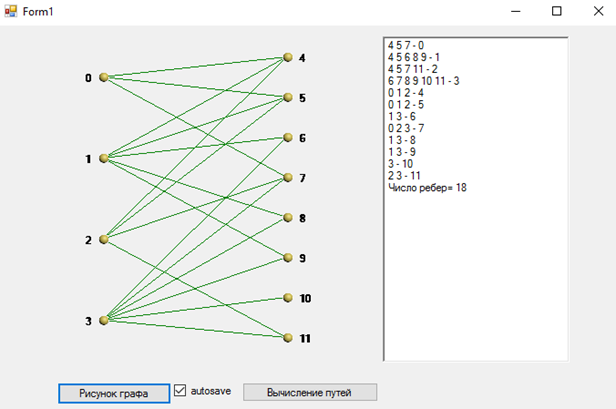
\includegraphics[width=350pt]{Fig1a}
  \caption{Исходный граф является двудольным.}\label{MAM_Fig1a}
\end{figure}
\par\medskip
\begin{figure}[h]
  %\centering
  % Requires \usepackage{graphicx}
  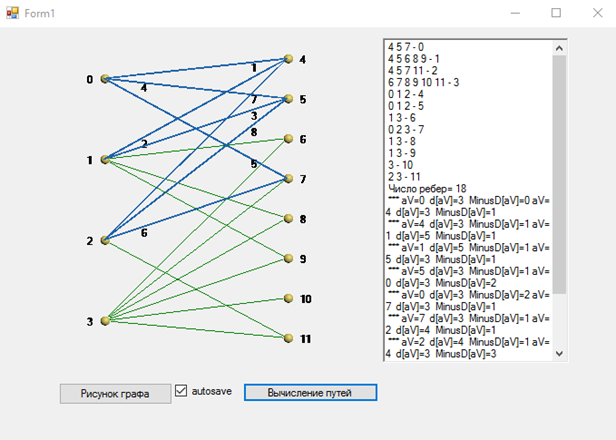
\includegraphics[width=350pt]{Fig1b}
  \caption{Созданы непродолжимые пути 0-4-1-5-0-7-2-4 и 2-5.}\label{MAM_Fig1b}
\end{figure}
\par\medskip
\begin{figure}[h]
  %\centering
  % Requires \usepackage{graphicx}
  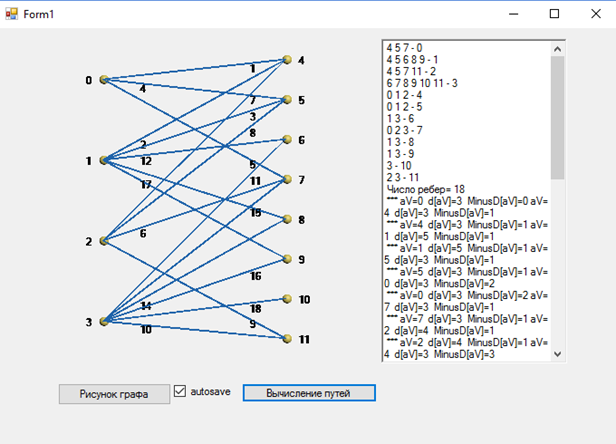
\includegraphics[width=350pt]{Fig1c}
  \caption{Построение разбиения завершено.}\label{MAM_Fig1c}
\end{figure}
\par\medskip
Заметим, что другим подходом к решению может быть классический обход графа. Обход вершин (ребер) графа в глубину и ширину может быть кратко сформулирован следующим образом:

произвольно выберем вершину (ребро), пометим $m=1$ и поместим в структуру $Т$ (список – в ширину, стек – в глубину); пока $Т$ не пусто, извлечем из нее вершину, затем каждую смежную ей непомеченную вершину пометим инкрементированным значением $m$ и поместим в $Т$.

Приведем рабочий код на языке Паскаль без деталей (и с тривиальными начальными данными для целей тестирования).
\begin{verbatim}
const
  n=2;
var
  i, k: integer;
  s: array [0..n-1] of set of byte =([2,3], [10,12]);
  count: integer=0;
begin
  for i := Low(s) to High (s) do
     for k := 0 to 255 do if k in S[i] then
      begin
         asm push k end;  inc (count)
      end;
  repeat
    asm pop k; end; Writeln (k); dec (count);
  until Count=0;
  readln;
end.
\end{verbatim}

\section{Ретроспективный прогноз}
Пусть о хронологии множества $V$ из $n$ событий сохранилась частичная информация: для некоторых пар событий $(u,v)$ известно, что событие $v$ произошло раньше события $u$ (запись $v<<u$). Ретроспективным прогнозом назовем такую сюръекцию $lbl$:
$V\rightarrow\{1,2,…, n\}$, что $lbl(v)<lbl(u)$ для каждого $v<<u$.

\underline{Алгоритм построения ретроспективного прогноза}. Построить ациклический орграф $G=(V,E)$ на $n$ вершинах так, что наличие в $E$ дуги $(u,v)$ соответствует $u<<v$, и выполнить помечивание $m(v):=0$ для всех $v$ из $V$. Пока множество
 $E$ не пусто:

а) выбрать вершину $v$ с нулевой полустепенью и дугу $(u,v)$;

б) $m(u):=max (m(u), m(v)+1)$;

в) удалить дугу $(u,v)$ из $E$;

г) если для $v$ полустепень захода равна нулю, удалить вершину $v$.

Восстановить граф $G=(V,E)$, упорядочить $V$ по неубыванию $m(v)$ и сопоставить каждой вершине $v$ значение $lbl(v)$, равное позиции вершины $v$ в упорядочении.

По заданной частичной информации программа генерирует ретроспективный прогноз, сопровождая каждый шаг пояснительной иллюстрацией.
Программа \cite{akm-prog2} предназначена для генерации непротиворечивого прогноза о полной хронологизации событий по заданной частичной информации о предшествовании. Рекомендуется использовать на занятиях по дискретной математике и/или компьютерной графике.
Цель программы – выполнить непротиворечивый прогноз о полном упорядочении событий по заданной информации о предшествовании, обеспечить выбор ручного и автоматического режимов управления визуализацией пошагового выполнения алгоритма. На рис.\ref{MAM_Fig2a}, \ref{MAM_Fig2b} и \ref{MAM_Fig2c} изображены начальный, промежуточный и завершающий этапы работы программы.

Характеристики программы:

среда и язык программирования: Microsoft .NET Framework 4.5, C\#;
тип ЭВМ – IBM PC;
операционная система – Windows 7.0, 8.1, 10.0;
объем программы – 319 КБ.

\begin{figure}[h]
  %\centering
  % Requires \usepackage{graphicx}
  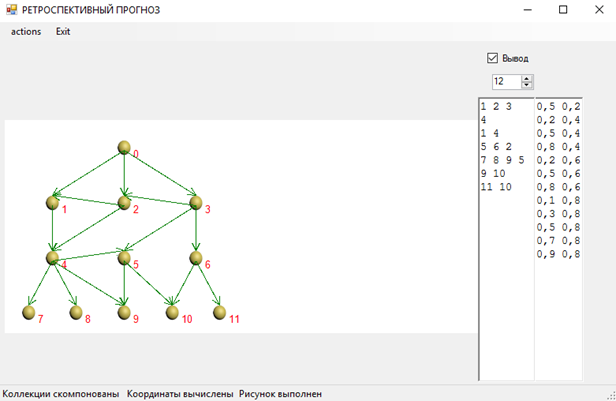
\includegraphics[width=350pt]{Fig2a}
  \caption{Исходный ациклический ориентированный граф.}\label{MAM_Fig2a}
\end{figure}
\par\medskip
\begin{figure}[h]
  %\centering
  % Requires \usepackage{graphicx}
  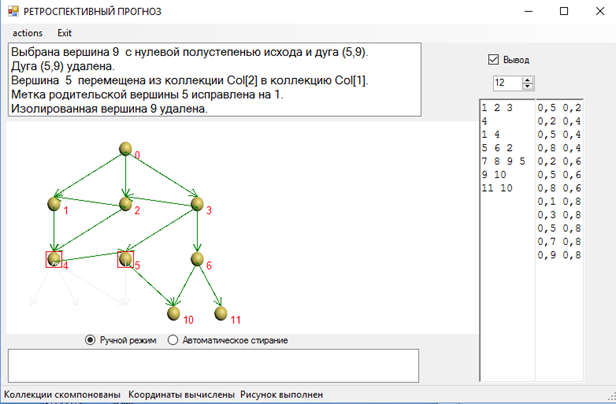
\includegraphics[width=350pt]{Fig2b}
  \caption{Начат процесс помечивания.}\label{MAM_Fig2b}
\end{figure}
\par\medskip
\begin{figure}[h]
  %\centering
  % Requires \usepackage{graphicx}
  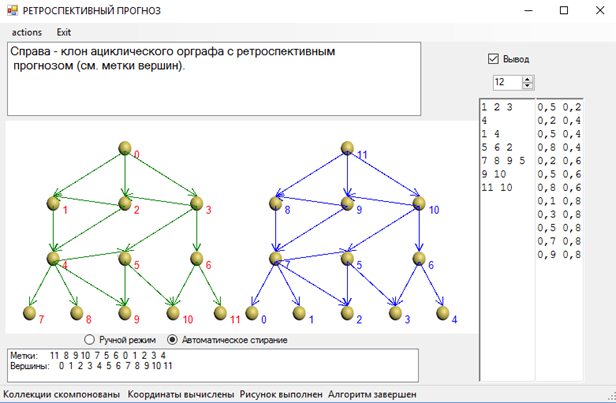
\includegraphics[width=350pt]{Fig2c}
  \caption{Процесс помечивания завершен.}\label{MAM_Fig2c}
\end{figure}
\par\medskip
\section{Процедура заливки фигур с ограничивающим цветом}
Процедура \cite{akm-prog3}
$$\small
FloodFill (Bitmap b, Color FillColor, Color BorderColor, int x, int y, int d)
$$
предназначена для заливки некоторой области $Q$ холста объекта $b$ цветом FillColor, начиная с точки $(x,y)$. В качестве границы области заливки $Q$ выступают точки заданного цвета BorderColor.

\underline{Дополнительное свойство}: процедура игнорирует различие цветов точек (и заливка просачивается через точки границы), если разница между соответствующими составляющими цветов $(R, G, B)$ точек не превышает значение последнего параметра $d$. См. рис.\, \ref{MAM_Fig3a} и \ref{MAM_Fig3b}.

В языке c\# данная процедура отсутствует среди стандартных. Цель: восполнить инструментарий программиста, включив функцию, отсутствующую среди стандартных функций языка c\#. При этом – снабженную дополнительным свойством по сравнению с аналогичными функциями других языков программирования.

Процедура востребована для программистов, для которых рабочим языком ранее являлся, например, язык Delphi; она найдет применение также и в преподавании языка c\# ввиду лаконичности и простоты изложения; к тому же ее алгоритм выгодно отличается от аналогичных алгоритмов, известных из электронных источников, тем, что вместо рекурсивного алгоритма с известной проблемой переполнения стека использована очередь (Queue) точек, подлежащих заливке; точки, подлежащие заливке, заносятся в очередь по принципу поиска в ширину.


Характеристики программы:

среда и язык программирования: Microsoft .NET Framework 4.5, C\#;
тип ЭВМ – IBM PC;
операционная система – Windows 7.0, 8.1, 10.0;
объем программы – 201 КБ.

\begin{figure}[h]
  %\centering
  % Requires \usepackage{graphicx}
  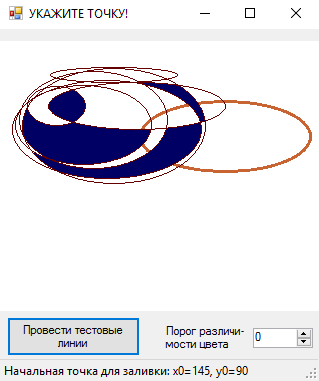
\includegraphics[width=250pt]{Fig3a}
  \caption{Параметр $d$ выбран равным нулю, поэтому заливка проникает сквозь границу.}\label{MAM_Fig3a}
\end{figure}
\par\medskip
\begin{figure}[h]
  %\centering
  % Requires \usepackage{graphicx}
  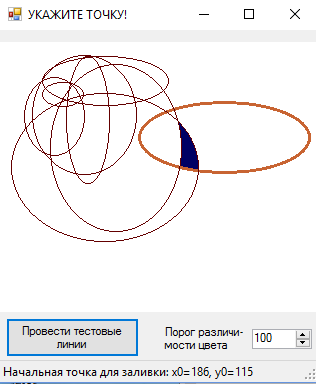
\includegraphics[width=250pt]{Fig3b}
  \caption{Параметр $d$, ответственный за непроницаемость границы, выбран отличным от нуля}\label{MAM_Fig3b}
\end{figure}
\par\medskip
\section{Реберная раскраска двудольных графов}
В теории расписаний востребованы теоретико-графовые представления задач; например, задача о составлении расписания обработки набора заданий в мультипроцессорной системе задается в виде двудольного графа, где наличие ребра $(u,v)$ означает предписание процессору $u$ выполнить обработку задания $v$ в течение промежутка единичной длительности.

В случае расписания без условий предшествования, с требованием работы каждого процессора без простоя и выполнения каждого задания без прерывания задача сводится к задаче интервальной реберной раскраски двудольного графа, которая, как известно, является NP-полной. Поэтому актуальна разработка эффективных эвристических алгоритмов поиска интервальной реберной раскраски для графов такого рода.
Программа предназначена для поиска интервальной реберной раскраски заданного двудольного графа, т.е. поиска такого отображения множества ребер графа в множество целых чисел (целое число – обозначение цвета), что для каждой вершины v множество цветов ребер, инцидентных $v$, образует некоторый целочисленный интервал. В основе алгоритма лежит разновидность метода полного перебора с возвратами, когда раскраска очередного ребра выполняется с соблюдением свойства интервальности цветов в каждой вершине.

Программу \cite{akm-prog4} рекомендуется использовать в разработке мультипроцессорных расписаний без простоев процессоров и прерывания выполнения заданий.
Цель программы – найти один из допустимых способов интервальной реберной раскраски заданного двудольного графа. Скриншот рис.\,\ref{MAM_Fig4a} дает определенное представление о формате выходного результата (правое окно) и промежуточных шагах (левое окно).

Характеристики программы:

среда и язык программирования: Microsoft .NET Framework 4.5, C\#;
тип ЭВМ – IBM PC;
операционная система – Windows 7.0, 8.1, 10.0;
объем программы – 196 КБ.
 %\begin{minipage}[t]{0.99\hsize}
\begin{figure}[h]
  %\centering
  % Requires \usepackage{graphicx}
  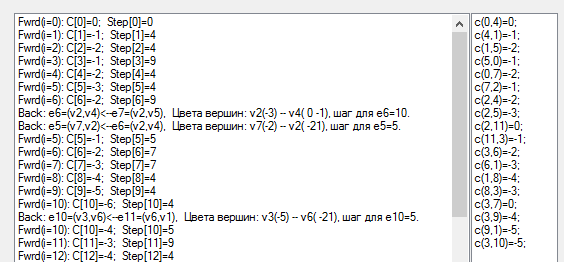
\includegraphics[width=250pt]{Fig4a}
  \caption{Справа программа поместила информацию об интервальной раскраске, в левом окне заметны прямые и обратные шаги процедуры поиска.}\label{MAM_Fig4a}
\end{figure}
%\end{minipage}
\par\medskip
\section{Генерация графов и их раскраска методом жадного алгоритма}
Функциональность программы \cite{akm-prog5} носит комплексный характер и состоит из двух частей:

1) интерактивный способ задания и отображения двудольного графа $G=(X,Y,E)$: чтение информации о списках смежности вершин графа из файла или конструирование ее программным путем, опция горизонтального или вертикального расположения вершин множеств $X$ и $Y$ и задание их мощностей и множества ребер $E$, сопровождение вершин надписями, загружаемыми в виде рисунков, а также сохранение изображения графа на любой стадии обработки;

2) генерация цепочечной структуры перечисления ребер графа, способствующей элиминации перебора на этапе раскраски, и собственно проверка существования раскраски – такого отображения $f$ множества ребер $E$ в множество целых
чисел (<<цвета>>), что для каждой вершины графа образы отображения $f$, полученные для инцидентных вершине <<раскрашенных>> ребер, попарно различны и образуют целочисленный интервал.
Программа предназначена главным образом для генерации графов и проверке существования их реберной раскраски.

Использованный метод: принцип жадного алгоритма – на любом этапе алгоритма выполненная часть отображения $f$ такова, что в каждой вершине v цвета раскрашенных ребер, инцидентных этой вершине, образуют целочисленный интервал.
Программу рекомендуется использовать в качестве программного обеспечения сопровождения выполнения выпускных квалификационных работ бакалавров и магистрантов по тематике теории графов и теории расписаний.
Цель программы: интерактивная генерация двудольных графов с визуализацией и проверкой существования реберной раскраски. На рис.\,\ref{MAM_Fig5a} (слева) программа отобразила найденную реберную раскраску.


Характеристики программы:

среда и язык программирования: Microsoft .NET Framework 4.5, C\#;
тип ЭВМ – IBM PC;
операционная система – Windows 7.0, 8.1, 10.0;
объем программы – 647 КБ.

\begin{figure}[h]
  %\centering
  % Requires \usepackage{graphicx}
  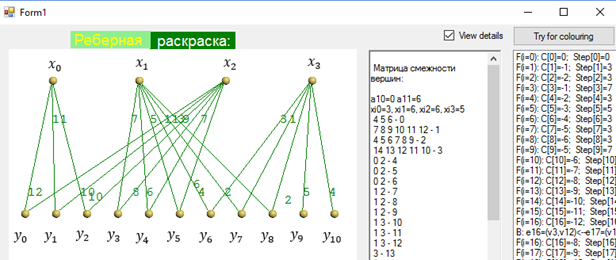
\includegraphics[width=250pt]{Fig5a}
  \caption{Сгенерирована интервальная реберная раскраска отображена метками ребер.}\label{MAM_Fig5a}
\end{figure}

\par\medskip

\section{Заключение}
Все составляющие программного обеспечения прошли тщательное тестирование. Программное обеспечение может быть использовано в учебном процессе направления <<Фундаментальная информатика и информационные технологии>>. Перспективным представляется разработка алгоритмов и компьютерных программ, способных однозначно ответить на вопрос о существовании реберной интервальной раскраски заданного графа. Приведенное выше программное обеспечение при тестировании показало надежность около 84 процентов.
